%!TEX root = ../main.tex

\chapter{Neue Version}
Wie in Abbildung \ref{fig:blockdiagramm} zu sehen ist, besteht die Platine aus mehreren Komponenten.
In Rot ist die Spannungsversorgung zu sehen, in Blau sind alle weiteren Verbindungen markiert und jeweils beschriftet.
Diese werden im Folgenden Kapitel näher erläutert, sowie die Schaltung und das Layout der Platine beschrieben.

\begin{figure}[H]
    \centering
    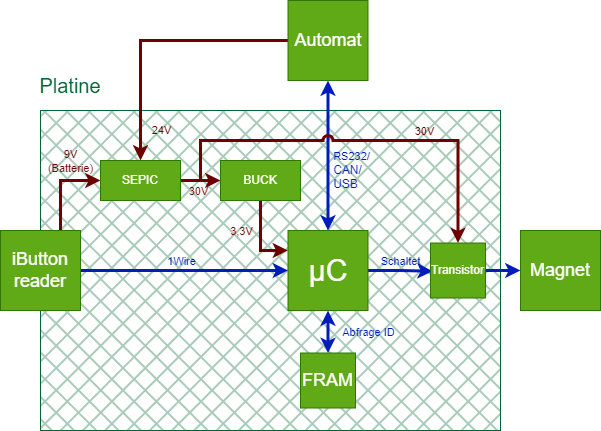
\includegraphics[width=1\textwidth]{resources/images/Blockdiagram.png}
    \caption[Blockdiagram]{Vereinfachte Darstellung der Funktion des Eschlosses}
    \label{fig:blockdiagramm}
\end{figure}

\section{Auswahl wichtiger \acp{IC}}
Bevor eine Schaltung realisiert werden kann, müssen die einzelnen Komponenten ausgewählt werden. Für verschiedene Bauelemente
gibt es unterschiedliche Anforderungen, die erfüllt werden müssen. Mit diesen Kriterien werden die am besten passenden
Bauteile ausgewählt. Dabei muss darauf geachtet werden, dass die Bauteile auch zusammen funktionieren.

Unabhängig von den individuellen Anforderungen müssen alle Bauteile folgende Kriterien erfüllen:
\begin{itemize}
    \item \textbf{Verfügbarkeit:} Die Bauteile müssen in ausreichender Stückzahl verfügbar sein.
    \item \textbf{Preis:} Die Bauteile müssen in einem angemessenen Preisrahmen liegen.
    \item \textbf{Lieferzeit:} Die Bauteile müssen in einer angemessenen Zeit lieferbar sein.
    \item \textbf{Dokumentation:} Die Bauteile müssen ausreichend dokumentiert sein.
    \item \textbf{Einfachheit:} Aus Grund der Einfachheit und aus Zeitgründen werden bereits in
          der Vergangenheit von krauth verwendete Bauteile bevorzugt. Vor allem diese, die bereits in
          der Bibliothek des verwendeten Layoutprogramms vorhanden sind.
\end{itemize}

In diesem Kapitel werden die wichtigsten Bauteile vorgestellt und die Auswahl anhand der wichtigsten Kriterien begründet.

\subsection{Microcontroller}
Der Microcontroller ist die zentrale Steuereinheit auf der Platine und damit das Herzstück des Systems. Die Auswahl
des Microcontrollers ist aus diesem Grund von großer Bedeutung und alle anderen Komponenten müssen an diesen
angepasst werden, daher muss dessen Auswahl als Erstes erfolgen.

Aktuell wird einen \enquote{MB9AF311k} von Spansion im E-Schloss verwendet, dieser ist jedoch am Ende seines
Produktlebenszykluses und wird daher in Zukunft nicht mehr verfügbar sein.

Die wichtigsten Kriterien für die Auswahl waren:
\begin{itemize}
    \item \textbf{Architektur:} Die Architektur des Microcontrollers muss zu der bereits vorhandenen Software passen.
    \item \textbf{Schnittstellen:} Die Schnittstellen des Microcontrollers müssen zu den vorhandenen Bauteilen passen.
    \item \textbf{Speicher:} Der Speicher des Microcontrollers muss ausreichend groß sein.
\end{itemize}

Nicht ausschlaggebend, aber dennoch gerne gesehen sind:
\begin{itemize}
    \item \textbf{\ac{USB}:} Die alte Version hatte eine \ac{USB} Schnittstelle vorgesehen, die jedoch nicht
          bestückt und verwendet wurde. In Zukunft soll diese Schnittstelle jedoch verwendet werden,
          aus diesem Grund ist es von Vorteil, wenn der Microcontroller bereits eine \ac{USB}
          Schnittstelle besitzt.
    \item \textbf{\ac{CAN}:} Aktuell gibt es keine \ac{CAN} Verbindung zwischen Automat und E-Schloss, mittlerweile ist
          dies jedoch der Standard. Eine \ac{CAN} Schnittstelle ist daher von Vorteil, vor allem für
          Zukunftssicherheit und Erweiterbarkeit.
\end{itemize}

Da die Firma STMicroelectronics bereits in der Vergangenheit von krauth verwendet wurde und die Software auf der
Architektur von STMicroelectronics basiert, ist es sinnvoll auch in Zukunft auf diese Firma zu setzen.
Außerdem ist die Dokumentation von STMicroelectronics sehr gut und es werden verschiedene Softwarepakete zur
Verfügung gestellt, die die Entwicklung vereinfachen können. \\
STMicroelectronics gibt eine Garantie von 10 Jahren auf die Verfügbarkeit der Microcontroller, womit auch eine
gewisse Zukunftssicherheit gegeben ist.

Die \enquote{STM32F0} Serie von STMicroelectronics ist eine kostengünstige Serie von Microcontrollern, die
die genannten Anforderungen erfüllen können. Weiter fiel die Wahl auf die \enquote{STM32F0x2} Unterserie, da
diese eine \ac{USB} und eine \ac{CAN} Schnittstelle besitzt. Von den übrigen Microcontrollern hat der
\enquote{STM32F072C8T6} sowohl eine passende Speichergröße, als auch eine angemessene Anzahl an Pins für die
Anwendung in diesem Projekt.
\clearpage

Der neu ausgewählte Microcontroller, der STM32F072C8T6 von STMicroelectronics steht nun gegen den alten
MB9AF311k von Spansion, den Vergleich der beiden Microcontroller ist in Tabelle \ref{tab:mcuVergleich} zu sehen.

\begin{table}[H]
    \centering
    \begin{tabular}{|l|l|l|}
        \hline
        \textbf{Microcontroller} & \textbf{MB9AF311k}     & \textbf{STM32F072C8T6} \\
        \hline
        \textbf{Hersteller}      & Spansion               & STMicroelectronics     \\
        \hline
        \textbf{Architektur}     & ARM Cortex M3          & ARM Cortex M0          \\
        \hline
        \textbf{Prozessortakt}   & 40MHz                  & 48MHz                  \\
        \hline
        \textbf{Flash Speicher}  & 64kB                   & 64kB                   \\
        \hline
        \textbf{\acs{RAM}}       & 16kB                   & 16kB                   \\
        \hline
        \textbf{Schnittstellen}  &
        \acs{I2C}                & \acs{I2C}                                       \\
                                 & \acs{USB}              & \acs{USB}              \\
                                 & \acs{UART}             & \acs{USART}            \\
                                 & \acs{CSIO} (\acs{SPI}) & \acs{SPI}              \\
                                 & \acs{LIN}              & \acs{CAN}              \\
        \hline
        \textbf{Programmierung}  & \acs{JTAG}             & \acs{SWD}              \\
        \hline
    \end{tabular}
    \caption{Vergleich der Microcontroller}
    \label{tab:mcuVergleich}
\end{table}

\subsection{\ac{SEPIC} Wandler}
Entweder die 24V automateninterne Spannung oder die ca.9V Batteriespannung, die bei Stromausfall an das
OneWire Terminal angeschlossen werden müssen auf 30V hochgeregelt werden.

Für diese Aufgabe wird ein \ac{SEPIC} Wandler verwendet. Ein \ac{SEPIC} Wandler wird verwendet, da dieser
ein sehr effizienter Aufwärtsregler ist, der auch bei geringen Eingangsspannungen funktioniert. Ein Vorteil
dieser Topologie ist das galvanische trennen von Ein- und Ausgangsspannung, was für die Sicherheit von Vorteil ist,
vor allem für \enquote{inrush currents}, also hohen Strömen beim ruckartigem Anschließen von Spannungsquellen,
die sich negativ auf die dahinter liegende Schaltung auswirken können.

Texas Instruments bietet viele verschiedene Schaltregler an, von denen bei krauth technology bereits einige
verwendet wurden. Da die Schaltregler von Texas Instruments sehr gut dokumentiert sind und bereits Erfahrung
mit diesen Bauteilen vorhanden ist, wird auch in diesem Projekt ein Modell dieser Firma verwendet. \\
Die Simulationssoftware von Texas Instruments, \enquote{Webench Designer}, bietet die Möglichkeit, die
Schaltung zu simulieren und die benötigten Bauteile zu berechnen, außerdem stehen andere
Simulationsmögligkeiten für Regler dieses Herstellers zur Verfügung. Das vereinfacht die Entwicklung und
spart Zeit.

Die Wahl ist auf den \enquote{LM5157} gefallen, der alle Anforderungen erfüllt und durch weiter funktionieren
wie eine weite Eingangsspanne und eine hohe Effizienz überzeugt. Zusätzlich verfügt das Gerät über integrierte
Schutzfunktionen wie Überspannungsschutz, Leitungs-UVLO, thermische Abschaltung und wählbaren Überlastschutz
im Hiccup-Modus. Zu den weiteren Merkmalen gehören ein niedriger Abschaltwert I Q, ein programmierbarer Softstart 
und eine externe Taktsynchronisation.

\subsection{Buck Wandler}
Die 30V Ausgangsspannung des \ac{SEPIC} Wandlers müssen auf 3,3V heruntergeregelt werden, um den Microcontroller
und die anderen Bauteile zu versorgen. Dafür wird ein Buck Wandler verwendet. Im Gegensatz zu einem Linerraregler
der aktuell verwendet wird, ist ein Buck Wandler deutlich effizienter, vor allem bei den größeren Spannungsunterschieden
die durch die neue Spannungsversorgung entstehen. Durch einen höheren Wirkungsgrad wird weniger Energie in Wärme
umgewandelt und der Wandler muss weniger Wärme abführen, was die Kühlung vereinfacht.

Da die Spannung 3,3V so weit verbreitet ist, gibt es einige Bauteile, die direkt diese Spannung ausgeben können.
Das verringert den benötigten Platz auf der Platine, indem kein Spannungsteiler zur Einstellung der Ausgangsspannung
ausgelegt werden muss.

Ein Wandler mit passender Eingangsspannungsspanne und adäquatem Ausgangsstrom bei den festen gewünschten 3,3V ist der
\enquote{AP63203WU-7} von Diodes Incorporated.

\subsection{RS-232 Treiber}
Für die RS-232 Schnittstelle wird ein Treiber benötigt, da der Microcontroller nicht direkt mit der Spannung der
Schnittstelle arbeiten kann. \\
Es gibt viele verschiedene Treiber auf dem Markt, die für diese Aufgabe verwendet werden können, da RS-232 ein
sehr verbreiteter Standard ist. Sie unterscheiden sich in der Anzahl der Kanäle, der benötigten Versorgungsspannung
und der maximalen Datenrate. Abgesehen davon haben die meisten Treiber ähnliche Eigenschaften und sind daher
austauschbar.

Bei diesem Gerät wird wieder auf einen Treiber von Texas Instruments gesetzt, da dieser bereits in der Vergangenheit
verwendet wurde und sehr gut auf die Anforderungen passt. Der \enquote{MAX3221} wird bereits in der alten Version
verbaut und hat sich bewährt. Da dieser trotz seines Alters noch verfügbar ist, wird dieser auch in der neuen Version
verwendet.

Der Treiber hat einen Datenkanal und die maximale Datenrate beträgt \(250 kbps\), was für diese Anwendung ausreichend ist.
Mit einer Versorgungsspannung von 3,3V ist dieser Treiber perfekt für die Anwendung geeignet und kann direkt mit der
Spannungsversorgung des Microcontrollers verbunden werden. Der \(\pm\)15kV \ac{ESD} Schutz ist ein weiterer Vorteil
dieses Treibers. Des weiteres schaltet sich das Gerät bei fehlendem validem RS-232 Eingangssignal in den Stromsparmodus,
was die Effizienz weiter erhöht.

\subsection{\ac{CAN} Treiber}
Auch für die \ac{CAN} Schnittstelle wird ein Treiber benötigt, um die Übertragungs-Pegel nach \ac{CAN} Standard zu
erzeugen. \\
Auch hier gibt es viele verschiedene Treiber auf dem Markt, die sich ebenfalls in der benötigten Versorgungsspannung,
dem verbrauchtem Strom während der Übertragung und im Ruhezustand, sowie in verschiedenen Zusatzfunktionen wie Standby-Modi
unterscheiden.

Da die \ac{CAN} Schnittstelle in der alten Version nicht verwendet wurde, wird hier ein neuer Treiber benötigt.
Die Wahl fällt aus oben genannten Gründen wieder auf ein \ac{IC} von Texas Instruments. \\
Der \enquote{SN65HVD230} ist ein kostengünstiger Treiber, der alle Anforderungen erfüllt. Diser verfügt über zahlreiche
Schutzfunktionen wie Kurzschlussschutz, Erdungs- und Überspannungsschutz, sowie Übertemperaturschutz. Außerdem hat
dieser Treiber einen Standby-Modus, der den Stromverbrauch im Ruhezustand verringert.

\subsection{\ac{FRAM}}
Der \ac{FRAM} Speicher wird verwendet um Daten persistent zu speichern. Dazu gehören die erlaubten iButton IDs, die
das Schloss öffnen dürfen, sowie die Konfiguration des Schlosses, also alles, was über einen Neustart hinaus abrufbar
bleiben muss. \\
Auch bei \acp{FRAM} gibt es viele unterschiedliche Produkte auf dem Markt. Entscheidend sind hier vor allem die Größe
des Speichers, die benötigte Versorgungsspannung und die Schnittstelle. Ein weiterer wichtiger Punkt ist die
Geschwindigkeit, da der Speicher bei jedem Öffnen des Schlosses ausgelesen wird und die Öffnung nicht unnötig
verzögert werden soll.

Im Gegensatz zu dem \ac{FRAM} Speicher der Version 1.0, dem \enquote{MB85rs64} von Fujitsu, mit 8 x 8 kbit
Speicher wird nun ein neuer mit einer höheren Kapazität benötigt, da im Betrieb der alten Version der Speicher
knapp wurde. \\
Ein 8 x 32 kbit, oder 256 kbit, mit einer Versorgungsspannung von 3,3V und einer \ac{SPI} Schnittstelle ist
der \enquote{FM25V02A-G} von Cypress. Dieser Speicher hat eine maximale Datenrate von 40MHz, mehr als genug für
das E-Schloss V2.0. Mit seinem geringen Stromverbrauch und der hohen Lebensdauer ist dieser Speicher perfekt
geeignet, um auf der Platine verbaut zu werden.

\clearpage

\section{Schaltplan}
Alle ausgewählten Teile müssen logisch miteinander verbunden werden, dazu wird ein Schaltplan erstellt, der alle
Verbindungen zwischen den Bauteilen aufzeigt.

Dabei ist wichtig die, Anforderungen an die einzelnen Bauteile zu beachten, die in den Datenblättern gegeben sind und
die Bauteile entsprechend zu dimensionieren. Eine weitere wichtige Aufgabe ist es die Bauteile so anzuordnen, dass
funktionale Gruppen möglichst nah beieinander liegen und Verbindungen nicht chaotisch über den ganzen Schaltplan
verteilt sind. Dadurch wird eine Übersichtlichkei gewahrt, die die spätere Weiterentwicklung vereinfacht und
die Einarbeitungszeit in die Platine verringert.
\begin{figure}[H]
    \centering
    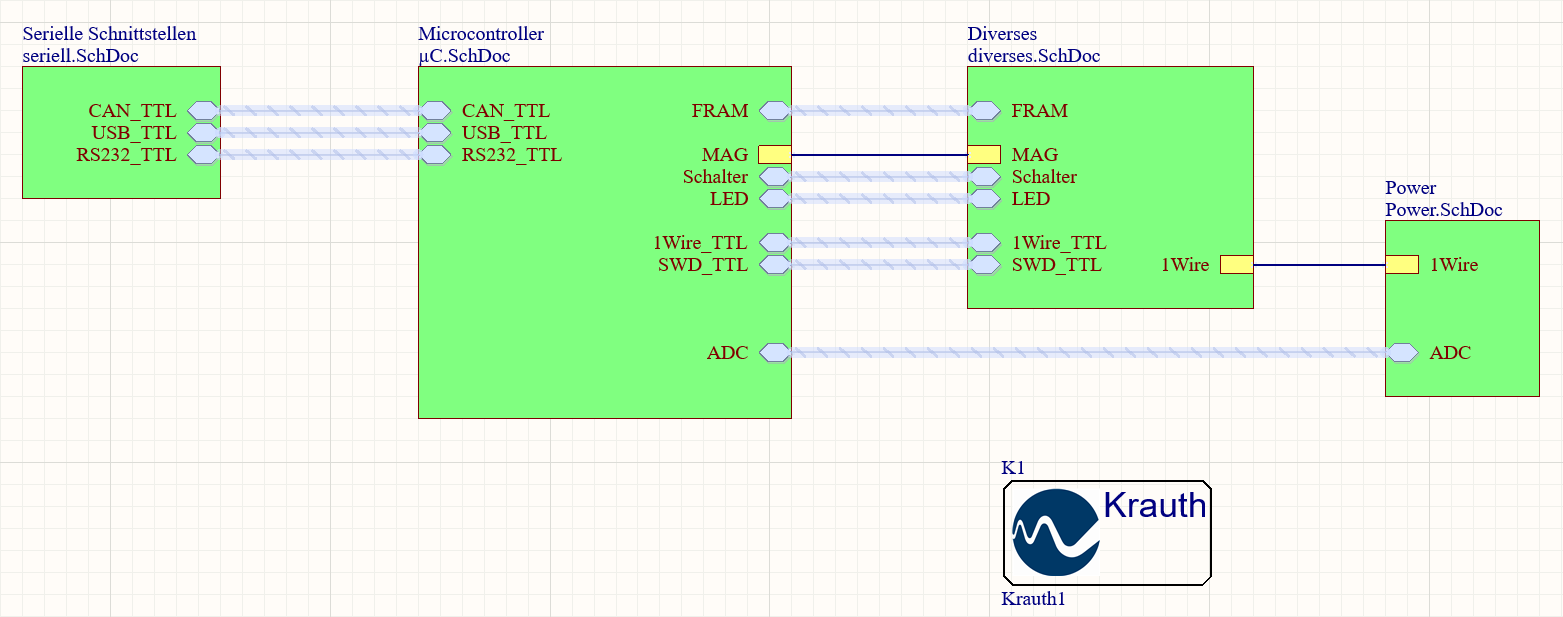
\includegraphics[width=1\textwidth]{resources/images/SP_Uebersicht.png}
    \caption[Schaltplan Übersicht]{Übersicht der Schaltpläne der Platine}
    \label{fig:sp_uebersicht}
\end{figure}
In Abbildung \ref{fig:sp_uebersicht} ist die Übersicht der einzelnen Schaltpläne und derer Verbindungen zu sehen.
Die hellblauen Verbindungen sind Kabelbäume aus thematisch zusammengehörigen Verbindungen und die gelb markierten
Leitungen sind einzelne Verbindungen. Alle Verbindungen sind mit einem Namen versehen, der die Funktion der Verbindung
beschreibt. \\
Wie in der Übersicht zu sehen ist, ist die Schaltung in mehrere Schaltpläne aufgeteilt, die jeweils eine
funktionale Gruppe darstellen. Diese sind in Abbildung \ref{fig:sp_uebersicht} mit einem grünen Rahmen markiert.

Im Folgenden werden die einzelnen Schaltpläne kurz beschrieben:
\begin{itemize}
    \item \textbf{seriell.SchDoc} beinhaltet die seriellen Schnittstellen, also \ac{USB}, \ac{CAN} und RS-232 mit ihren
          dazugehörigen Treibern, Schutzbeschaltungen und Adaptern.
    \item \textbf{µC.SchDoc} beinhaltet den Microcontroller und seine Stützkondensatoren, Debug Schnittstelle,
          die Quarze mitsamt Beschaltung und den Batteriehalter, um auch bei Stromverlust die \ac{RTC} zu versorgen.
    \item \textbf{Power.SchDoc} beinhaltet die Spannungsversorgung, also die beiden Schaltregler und die dazugehörigen
          Beschaltungen. Außerdem die Kondensatoren, die als Puffer für die Magneten dienen.
    \item \textbf{diverses.SchDoc} beinhaltet alle anderen Bauteile, darunter sind der \ac{FRAM} Speicher und verschiedene
          Stecker und Buchsen:
          \begin{itemize}
              \item \textbf{Magnet} Transistor um 30V auf Magneten zu geben
              \item \textbf{LEDs} mit Vorwiderständen und Schutzbeschaltung
              \item \textbf{IButton} mit Logik und Schutzbeschaltung
              \item \textbf{SWD} nur Buchse und Pull-Up Widerstände
              \item \textbf{Schalter} Anschluss für einen Endschalter am Schloss
          \end{itemize}

\end{itemize}
\subsection{Spannungsversorgung}
Die Spannungsversorgung ist ein wichtiger Teil der Schaltung, da alle anderen Bauteile mit Spannung versorgt werden müssen.
Die große Veränderung gegenüber Version 1.0 ist der Wechsel von einer 12V Versorgung auf eine 30V Versorgung. 

Über die Dioden D100 und D103 werden die beiden Spannungsquellen, also die 24V automateninterne Spannung und die
9V Batteriespannung zusammengeführt. Die Dioden verhindern dabei, dass die Spannung zur Beschaltung der jeweils anderen
Spannungsquelle fließen kann. Von Transistorschaltung um die Spannungsquelle zu wählen kann abgesehen werden, da die
Spannungen nicht gleichzeitig anliegen werden, eine Batterie wird nur angeschlossen, wenn der Automat keinen Strom hat.

Diese Eingangsspannungen müssen noch durch einige Bauteile gefiltert werden, um die Spannungsspitzen zu glätten und
die Spannung zu stabilisieren. Über die \ac{TVS} Diode D102 wird die Spannung auf 28V begrenzt, um die dahinter liegende
Schaltung vor Überspannung zu schützen. Der Kondensator C104 soll eventuelle Spannungsspitzen glätten. Des Weiteren
ist zwischen Eingang und \ac{SEPIC} Wandler eine Ferritperle FB100 eingebaut, um die Schaltung vor Störungen zu schützen.
Diese Ferritperle filtert die hochfrequenten Störungen durch den Schaltregler heraus, die durch das schnelle Schalten
entstehen und andere Teile der Schaltung stören können.

Nach der Filterung wird die Spannung durch den \ac{SEPIC} Wandler auf 30V hochgeregelt. Die Schaltung des \ac{SEPIC}
wird im Folgenden Kapitel genauer beschrieben. Auf der Ausgangsseite des \ac{SEPIC} Wandlers sind die Kondensatoren
C125, C126 und C127 mit einer Kapazität von jeweils \(2.200 \mu F\) verbaut, die als Energiespeicher während des
Betriebes mit Batteriespannung dienen. Diese Kondensatoren ersetzen 3 \(4.700 \mu F\) Kondensatoren aus der alten Version.
Durch die höhere Spannung wird somit fast die dreifache Menge an Energie gespeichert, was die Laufzeit des Schlosses
bei Batteriebetrieb deutlich erhöht. Um das zu zeigen wird folgende Formel verwendet:

\[E_{el} = \frac{1}{2} \times C \times U^2\]

\(E_{el}\) ist die gespeicherte Energie in Joule, \(C\) ist die Kapazität in Farad und \(U\) ist die Spannung in Volt.
Die Energie der alten Version beträgt damit \(E_{el} = 3 \times 0,5 \times 4.700 \mu F \times (12V)^2 = 1,01 J\) und die Energie der neuen
Version liegt bei \(E_{el} = 3 \times 0,5 \times 2.200 \mu F \times (30V)^2 = 2,97 J\).

Falls die gespeicherte Energie trotzdem nicht ausreichen sollte, kann diese durch den Stecker S100 mit weiteren Kondensatoren
erweitert werden.

\clearpage

\subsubsection{SEPIC Wandler}
Für die Auslegung des \ac{SEPIC} Wandlers wird die online verfügbare Software \enquote{Webench Designer} von Texas
zur Hilfe gezogen (Verfügbar unter \url{http://www.ti.com/design-tools/overview.html}). Dieses Werkzeug bietet die
Möglichkeit, die Schaltung zu simulieren und die benötigten Bauteile zu berechnen.

Für einen guten Überblick ist außerdem das Microsoft Excel Tool \enquote{LM5157 Quick start Calculator} (unter der url \url{
https://www.ti.com/tool/download/SNVR512} zu finden), welches ebenfalls von Texas Instruments ist, zum Einsatz gekommen. 
Dort kann schnell an einzelnen Parametern der Schaltung justiert werden und die Auswirkungen auf die Schaltung werden 
direkt errechnet.

Am Eingang des \ac{SEPIC} Wandlers sind die Kondensatoren C101, C102 und C103 verbaut, welche die Spannung glätten und die
schnellen Schaltspitzen des \ac{SEPIC} Wandlers abfangen. Die Werte dieser Kondensatoren sind in verschiedenen Größenordnungen
gewählt, um die Schaltspitzen über einen großen Frequenzbereich abzufangen.

\begin{figure}[H]
    \centering
    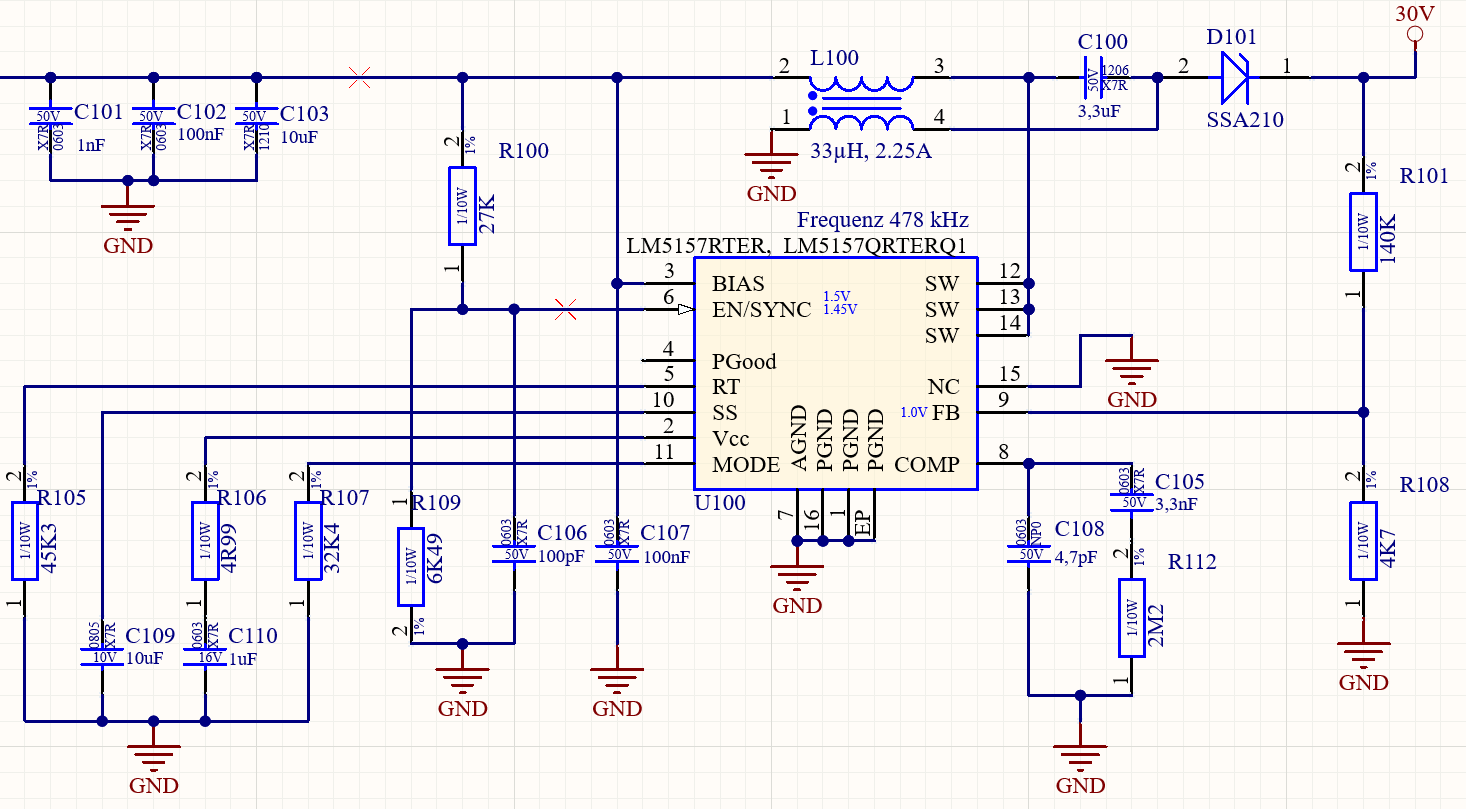
\includegraphics[width=1\textwidth]{resources/images/Sepic_sp.png}
    \caption[SEPIC Schaltung]{Schaltung des SEPIC Wandlers}
    \label{fig:sepic_sp}
\end{figure}

\paragraph{VCC Pin}\mbox{}\\
Aus dem Datenblatt des \enquote{LM5157} (siehe \cite{LM5157}) können die festen Parameter für \(R106 = 5\Omega\) und
\(C110 = 1\mu F\) entnommen werden. Diese Bauteile werden in Reihe gegen Masse an den VCC Pin (Versorgungsspannung)
angeschlossen.

\paragraph{Feedback Pin}\mbox{}\\
Die Widerstände R101 und R108, die als Spannungsteiler fungieren, werden so gewählt, dass die Ausgangsspannung
des \ac{SEPIC} Wandlers 30V beträgt. Die Werte der Widerstände werden mit folgender Formel berechnet (siehe
Datenblatt S.23 \cite{LM5157}):

\[U_{OUT} = U_{REF} \times \frac{R_{108}}{R_{101} + R_{108}}\]

Mit der geforderten Ausgangsspannung \(U_{OUT} = 30V\) und der Referenzspannung \\
\(U_{REF} = 1V\) (siehe Datenblatt) ergibt sich ein Verhältnis von 29:1 für die Widerstände \(R_{101}\) und \(R_{108}\).
Wählt man nun den Widerstand \(R_{101} = 140k\Omega\), muss der Widerstand \(R_{108} = 4,83k\Omega\) betragen um 
dieses Verhältnis zu erfüllen. Da es den besagten Widerstandswert so nicht zu kaufen gibt, wird der nächst kleinere 
Wert der Standardreihe \(R_{108} = 4,7k\Omega\) verwendet.

Damit liegt die tatsächliche Ausgangsspannung bei \(U_{OUT} = 30,1V\), was im Rahmen der Toleranz liegt und keines der dahinter
liegenden Bauteile beeinträchtigen sollte.

\paragraph{Undervoltage Lockour Pin}\mbox{}\\
Mit den Widerständen \(R_{100}\) und \(R_{109}\) wird ein weiterer Spannungsteiler realisiert, der die Spannung am
UVLO Pin des \enquote{LM5157} einstellt. Dieser Pin ist für die Unterspannungsabschaltung zuständig, die den Regler
abschaltet, wenn die Eingangsspannung unter einen bestimmten Wert fällt. Die Größen dieser Widerstände wird mit Folgenden
Formeln berechnet (siehe Datenblatt S.23 \cite{LM5157}):

\[\displaystyle
    R_{100} = \frac{V_{SUPPLY(ON)} \times
        \frac{V_{UVLO(FALLING)}}{V_{UVLO(RISING)}}
        - V_{SUPPLY(OFF)}}{I_{UVLO}}
\]

\[\displaystyle
    R_{109} = \frac{V_{UVLO(RISING)} \times R_{100}}{V_{SUPPLY(ON)} - V_{UVLO(RISING)}}
\]

Folgende Werte können so aus dem Datenblatt entnommen werden:
\begin{itemize}
    \item \(V_{UVLO(RISING)} = 1,5V\)
    \item \(V_{UVLO(FALLING)} = 1,45V\)
    \item \(I_{UVLO} = 5\mu A\)
\end{itemize}
Geht man dann von \(V_{SUPPLY(ON)} = 8V\) (Spannung, ab der der Regler sich einschalten soll) und \(V_{SUPPLY(OFF)} = 7,6V\)
(Spannung, unter welcher der Regler sich kontrolliert abschaltet) aus, so ergibt sich ein Wert von \(26,67k\Omega\) für den 
Widerstand R100, weshalb \(R_{100} = 27k\Omega\) gewählt wird. Mit diesen Werten in Formel zwei eingesetzt, errechnet sich
der Widerstandswert für \(R_{109}\) zu \(6,23k\Omega\), was auf \(R_{109} = 6,49k\Omega\) aufgerundet wird. \\
Damit ein kurzzeitiges Unterschreiten der Schwelle von \(V_{SUPPLY(OFF)}\) kein Problem darstellt, wird zusätzlich ein Kondensator
\(C_{106} = 100pF\) parallel zu \(R_{109}\) geschaltet.

\paragraph{Schaltfrequenz (RT Pin)}\mbox{}\\
Der Widerstand \(R_{105}\) am RT Pin stellt die Schaltfrequenz des Reglers ein. Der Widerstand berechnet sich durch folgende
Formel (siehe Datenblatt S.18 \cite{LM5157}):

\[R_{RT} = \frac{2,21 \times 10^{10}}{f_{RT}} - 955 \]

Durch die Senkung der Frequenz steigt die Effizienz des Reglers, da die Schaltverluste sinken. Allerdings steigt dadurch auch die
Größe der benötigten Spule. Nach evaluieren verschiedener Frequenzen wurde eine Frequenz von etwa \(f_{RT} = 480kHz\) gewählt, da 
diese einen guten Kompromiss zwischen Effizienz und Bauteilgröße darstellt. Mit dieser Frequenz ergibt sich ein Widerstand von 
\(R_{RT} = 45,1k\Omega\). Ein Widerstand nah an diesem Wert ist \(45,3k\Omega\), dieser wird hier verwendet.

Damit ergibt sich die Schaltfrequenz des Reglers \(f = 478kHz\), was auch auf dem Schaltplan in Abbildung \ref{fig:sepic_sp}
notiert ist. Um später im EMV-Labor oder bei anderweitiger Fehlersuche und Entstörung die Schaltfrequenz zu kennen.

\paragraph{Modus (Mode Pin)}\mbox{}\\
Der \enquote{LM5157} kann in vier verschiedene Modi geschaltet werden, indem verschiedene Widerstände zwischen Mode-Pin
und Masse verbunden werden. Die Modi sind in Tabelle \ref{tab:sepic_modes} aufgelistet. In der Schaltung wird der Widerstand
\(R_{107} = 37,4k\Omega\) verwendet, wodurch der Regler in den \ac{DRSS} und Hickup Modus geschaltet wird.

\begin{table}[H]
    \centering
    \begin{tabular}{|l|l|l|}
        \hline
        \textbf{Hickup} & \textbf{DSSR} & \textbf{Widerstand \(R_{107}\)} \\
        \hline
        Nein            & Nein          & \(0\Omega\)                      \\
        \hline
        Ja              & Ja            & \(37,4k\Omega\)                  \\
        \hline
        Ja              & Nein          & \(62k\Omega\)                    \\
        \hline
        Nein            & Ja            & \(100k\Omega\)                   \\
        \hline
    \end{tabular}
    \caption{Verschiedene Modi des LM5157}
    \label{tab:sepic_modes}
\end{table}

\ac{DRSS} ist eine Technik von Texas Instruments, die zur Reduktion von \ac{EMI} verwendet wird. Dabei wird die Schaltfrequenz
des Reglers variiert, um die Störungen zu verteilen und so die Störstrahlung zu reduzieren. \\
Eine niedrigfrequente zufällige dreieckige Variation der Schaltfrequenz wird mit einer hochfrequenten zufälligen Variation überlagert.
Die Störstrahlung wird dadurch auf ein breiteres Frequenzband verteilt und durch die zufällige Variation des dreieckigen Profiles
wird die Wahrscheinlichkeit von hörbaren Geräuschen reduziert. \\
(TI - Application Note DRSS \cite{drss})

\begin{figure}[H]
    \centering
    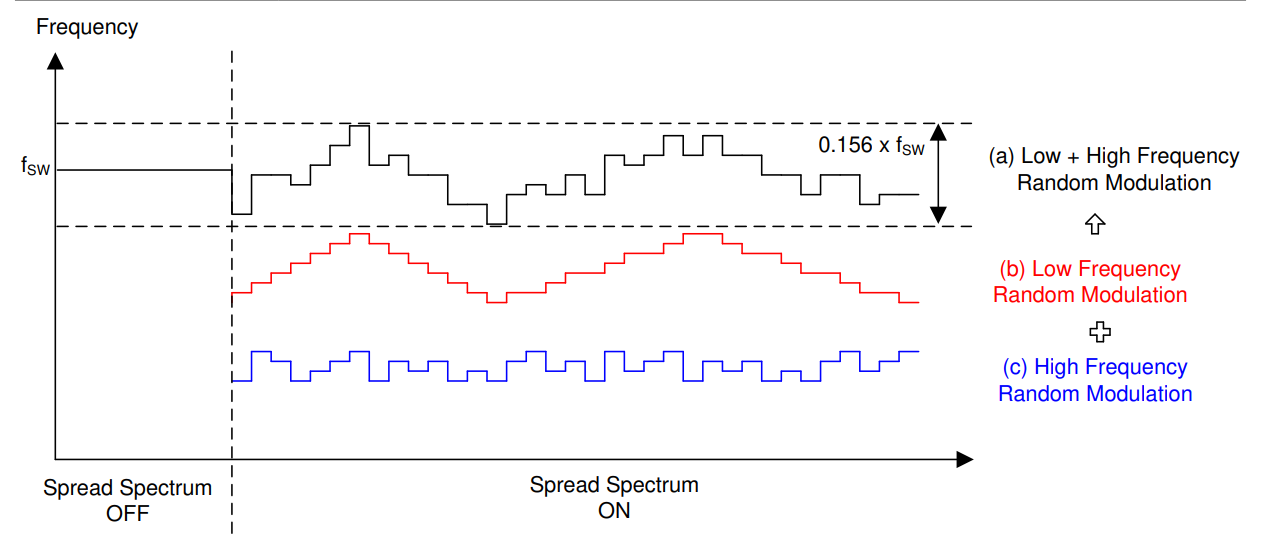
\includegraphics[width=1\textwidth]{resources/images/drss.png}
    \caption[DRSS]{DRSS Technik von Texas Instruments(S.19 Datenblatt\cite{LM5157})}
    \label{fig:drss}
\end{figure}

Hiccup Modus ist eine weitere Schutzfunktion, welche die Komponenten vor zu hohen Strömen schützt. Dabei schaltet sich der Regler
nach 64 aufeinanderFolgenden Schaltzyklen im Strombegrenzungsmodus ab und versucht sich nach einer kurzen Pause von
32768 Schaltzyklen wieder einzuschalten. Dieser Vorgang wird solange wiederholt, bis die Überlastung nicht mehr besteht.
Der 64 Zyklen Hiccup Timer wird zurückgesetzt, wenn der Strom für acht aufeinanderfolgende Schaltzyklen unter den Überlastwert sinkt. \\
(Siehe Datenblatt S.24 \cite{LM5157})

\begin{figure}[H]
    \centering
    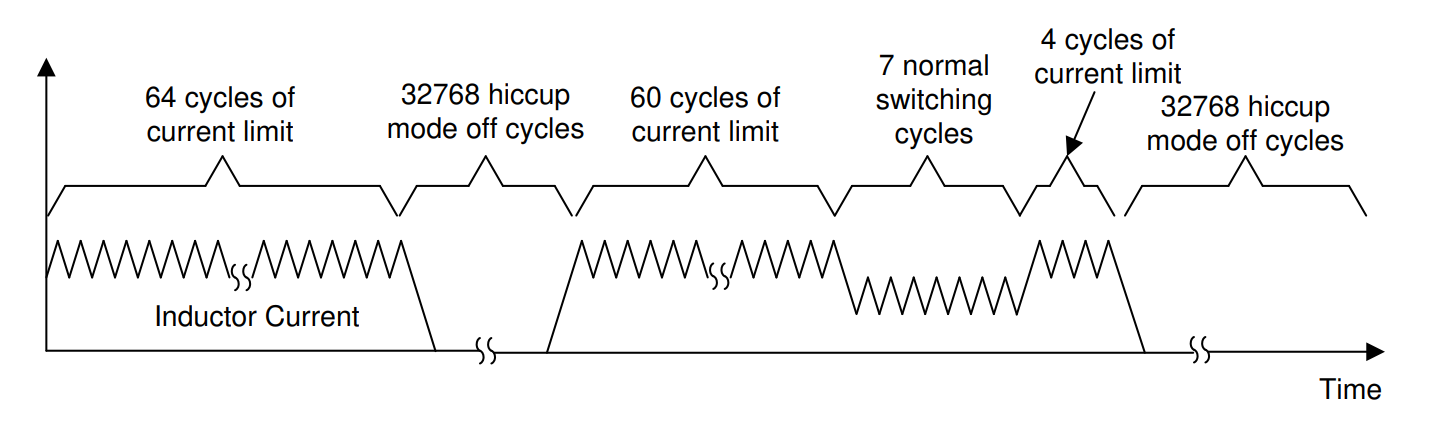
\includegraphics[width=1\textwidth]{resources/images/hiccup.png}
    \caption[Hickup]{Hiccup Technik von Texas Instruments(S.24 Datenblatt\cite{LM5157})}
    \label{fig:hiccup}
\end{figure}

\

\paragraph{Softstart (SS Pin)}\mbox{}\\
Über den Softstart Pin kann die Einschaltzeit des Reglers eingestellt werden. Dadurch wird die Einschaltstromspitze reduziert
und das System sicher gestartet. Der Feedback Pin des Gerätes wird entweder auf die Spannung an dem SS Pin, oder auf die
interne Referenzspannung geschaltet, je nach dem, was in diesem Moment das niedrigere Potential hat.

Die Zeit, die der Regler zum einschalten benötigt, wird durch folgende Formel berechnet (siehe Datenblatt S.17 \cite{LM5157}):

\[t_{SS} = \frac{C_{SS}}{I_{ss}} \times V_{REF}\]

\(I_{SS}\) ist dabei ein interner Softstart Strom von \(10\mu A\), der bei Überschreitung der \(U_{UVLO}\) Schwelle eingeschaltet
wird und den Einschaltvorgang startet. \(V_{REF}\) ist die interne Referenzspannung von \(1V\), damit ergibt sich eine Einschaltzeit
proportional zur Kapazität \(C_{SS}\). Pro \(1ms\) Einschaltzeit wird eine Kapazität von \(10nF\) benötigt. \\
Da eine große Kapazität am Ausgang des Reglers angeschlossen ist, wird hier ein Kondensator von \(C_{109} = 10\mu F\) verwendet, was
eine Einschaltzeit von \(1s\) ergibt. So wird sichergestellt, dass der Regler sicher startet und der Strom limitiert ist,
während die Kapazitäten geladen werden.

\paragraph{Loop Compensation (COMP Pin)}\mbox{}\\
Die Komponenten \(C_{105}\), \(C_{108}\) und \(R_{112}\) sind an den COMP Pin angeschlossen. Diese externen
Komponenten bilden ein Kompensationsnetzwerk, welches die Schleifenverstärkung des Regelkreises beeinflusst. Durch die 
richtige Auswahl dieser Komponenten kann die Stabilität und Leistung des Regelkreises optimiert werden, indem die 
Phasenverschiebung und die Verstärkung des Regelkreises beeinflusst und somit ungewollte Schwingungen verhindert werden.

\begin{figure}[H]
    \centering
    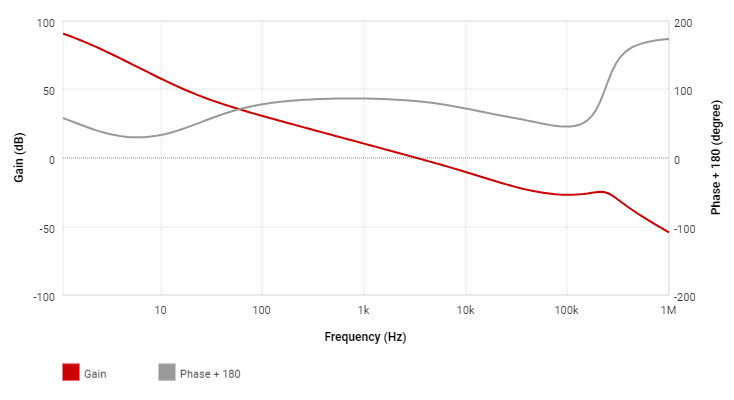
\includegraphics[width=1\textwidth]{resources/images/bode.png}
    \caption[Bode-Plot]{Bode-Plot der Regelkreisantwort des SEPIC Wandlers}
    \label{fig:bode}
\end{figure}

Die Werte für diese Komponenten wurden mit Hilfe des online Werkzeugs \enquote{Webench Designer} berechnet. Sie produzieren damit
Folgenden Bode-Plot als Regelkreisantwort (siehe Abbildung \ref{fig:bode}). Dies sind die errechneten Werte:
\begin{itemize}
    \item \(C_{105} = 3,3nF\)
    \item \(C_{108} = 4,7pF\)
    \item \(R_{112} = 2,2M\Omega\)
\end{itemize}
Damit ergibt sich eine Grenzfrequenz von \(f_{G} = 3,3Khz\), eine Phase Margin von \(PM = 83^\circ\) und ein Gain Margin
von \(GM = - 112dB\). Diese Werte sind für die Stabilität des Regelkreises ausreichend und sollten keine ungewollten Schwingungen
verursachen. \\
(Texas Instruments - Loop Compensation made easy \cite{comp})

\

\paragraph{Energiespeicher}\mbox{}\\
Als Energiespeicher werden die Doppeldrossel L100 und der Kondensator C100 eingesetzt. Der Induktivitätswert der Doppeldrossel
wird mit folgender Formel berechnet (Texas Instruments - Designing DC/DC convertors based on SEPIC topology \cite{sepic}):

\[L = \frac{1}{2} \times \frac{V_{IN} \times D_{MAX}}{\Delta I_L \times f_{SW(min)}}\]

Bei \(D_{MAX}\) handelt es sich um den maximalen Dutycicle des Reglers, der bei \(V_{min}\) auftritt. Diesen Wert kann man mit
folgender Formel berechnen:

\[D_{MAX} = \frac{V_{OUT} + V_{FWD}}{V_{IN} + V_{OUT} + V_{FWD}}\]

Bei diesem Design kommt man mit der Durchlassspannung der Diode \(V_{FWD} = 0,8V\) und der minimalen Eingangsspannung von
\(V_{IN(min)} = 8V\) auf einen Wert von \(D_{MAX} = 0,79\).

Mit einem festen Wert für den Rippelstrom der Drosselspule \(\Delta I_L = 0,2A\) und der Schaltfrequenz von \(f_{SW} = 478kHz\)
ergibt sich ein Wert von \(L = 33\mu H\) für die Induktivität L100.

\subsubsection{Buck Wandler}
Der Buck Wandler wird verwendet, um die 30V Ausgangsspannung des \ac{SEPIC} Wandlers auf 3,3V herunterzuregeln. Diese 3,3V Spannung
wird dann als Versorgungsspannung für den Microcontroller und die anderen \acp{IC} verwendet.

\begin{figure}[H]
    \centering
    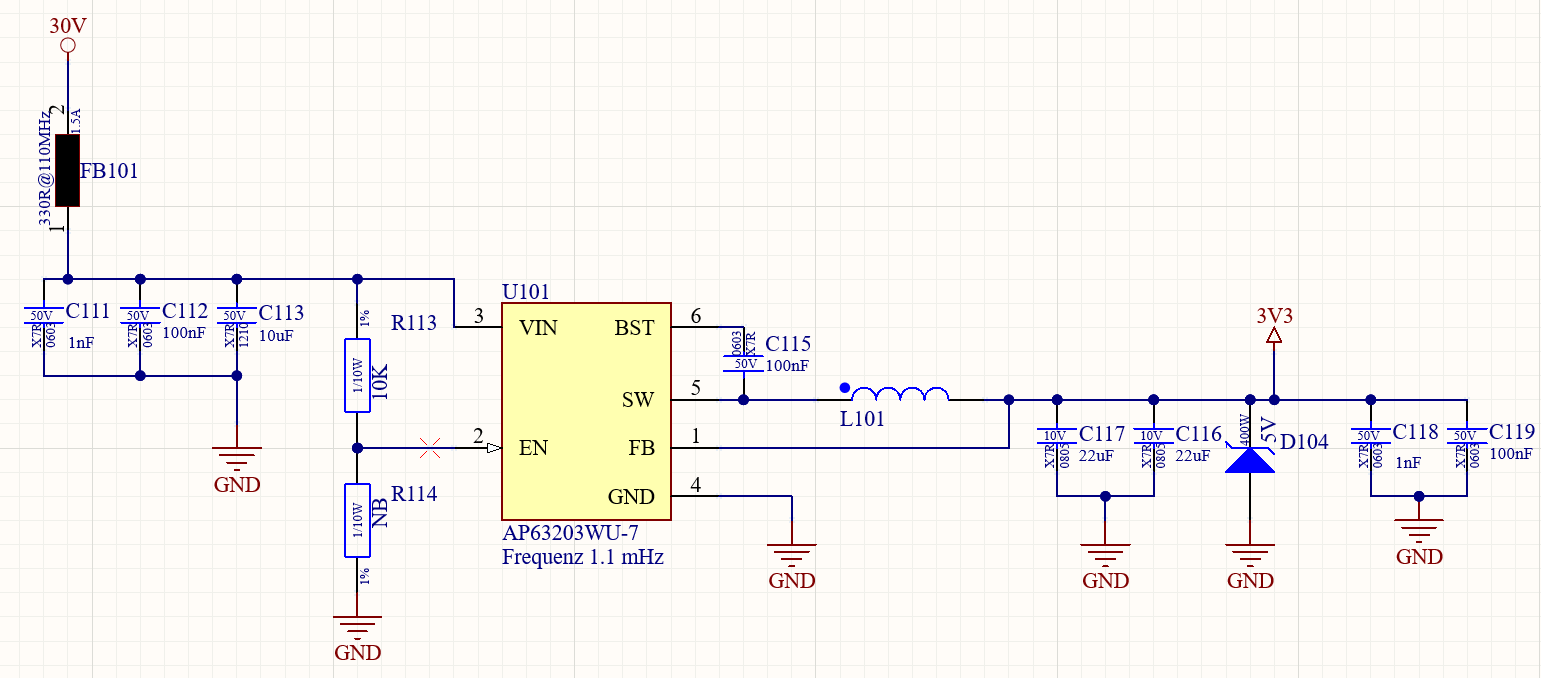
\includegraphics[width=1\textwidth]{resources/images/buck_sp.png}
    \caption[Buck Schaltung]{Schaltung des Buck Wandlers}
    \label{fig:buck_sp}
\end{figure}

Wie bei dem eben beschriebenen \ac{SEPIC} Wandler wird auch hier eine Ferritperle (FB101) verwendet, um die Schaltung vor Störungen
durch den Wandler zu schützen. Ebenfalls analog zu der Beschaltung des\ac{SEPIC} Wandlers werden die Kondensatoren C111, C112 und
C113 in verschiedenen Größenordnungen gewählt, um die Schaltspitzen über einen großen Frequenzbereich abzufangen.

Widerstand R114 ist nicht bestückt. Dieser Widerstand kann bei Bedarf verwendet werden um, zusammen mit R113 einen Spannungsteiler 
zu bilden, der die Einschaltspannung des Reglers einstellt. Die Formeln dafür sind in den Datenblättern der Regler zu finden 
\cite{AP63203WU}. Mit dem festen Wert von \(R_{113} = 10k\Omega\) kann man diese umstellen und nach \(R_{114}\) auflösen.

Als erstes wird der Wert für \(V_{OFF}\) berechnet:
\[V_{OFF} = 0,932 \times V_{ON} - 10k\Omega \times 4,1\mu A\]

Dann kann dieser in folgende Formel eingesetzt werden, um den Widerstandswert für \(R_{114}\) zu berechnen:
\[R_{114} = \frac{1,1 \times 10k\Omega}{V_{OFF} - 1,1V + 5,5\mu A \times 10k\Omega}\]

\paragraph{Werte aus dem Datenblatt}\mbox{}\\
Der Rest der Komponenten für diese Schaltung wird aus dem Datenblatt des \enquote{AP63203WU-7} entnommen. Da dieser Regler spezifisch
für die Anwendung mit 3,3V Ausgangsspannung entwickelt wurde, sind die Werte für die Kondensatoren und die Induktivität bereits
gegeben und ein Spannungsteiler für den Feedback Pin ist nicht nötig.
\begin{table}[H]
    \centering
    \begin{tabular}{|l|l|}
        \hline
        \textbf{Bauteil} & \textbf{Wert} \\
        \hline
        C115             & \(100nF\)     \\
        \hline
        L101             & \(9\mu H\)    \\
        \hline
        C116             & \(22\mu F\)   \\
        \hline
        C117             & \(22\mu F\)   \\
        \hline
    \end{tabular}
    \caption{Standartwerte für den AP63203WU-7 aus dem Datenblatt\cite{AP63203WU}}
    \label{tab:AP63203WU}
\end{table}

\paragraph{Schutz der Schaltung}\mbox{}\\
Um die Schaltung vor Überspannung zu schützen, wird eine \ac{TVS} Diode D104 verwendet, welche die Spannung auf 5V begrenzt.
Eine solche Spannung sollte niemals an dem Ausgang des Reglers anliegen, dennoch ist es wichtig die empfindlichen Bauteile
wie den Microcontroller ausreichend zu schützen.

\subsection{Anschlüsse des Microcontrollers}
Der Microcontroller als zentrale Steuereinheit des Schlosses muss mit vielen anderen Bauteilen verbunden werden. Wie in
Abbildung \ref{fig:uC_uebersicht} zu sehen ist, werden alle 48 Beine des Microcontrollers verwendet. Die Anschlüsse
und Schaltungen auf der Schaltplanseite des Microcontrollers werden im Folgenden kurz beschrieben.

\begin{figure}[H]
    \centering
    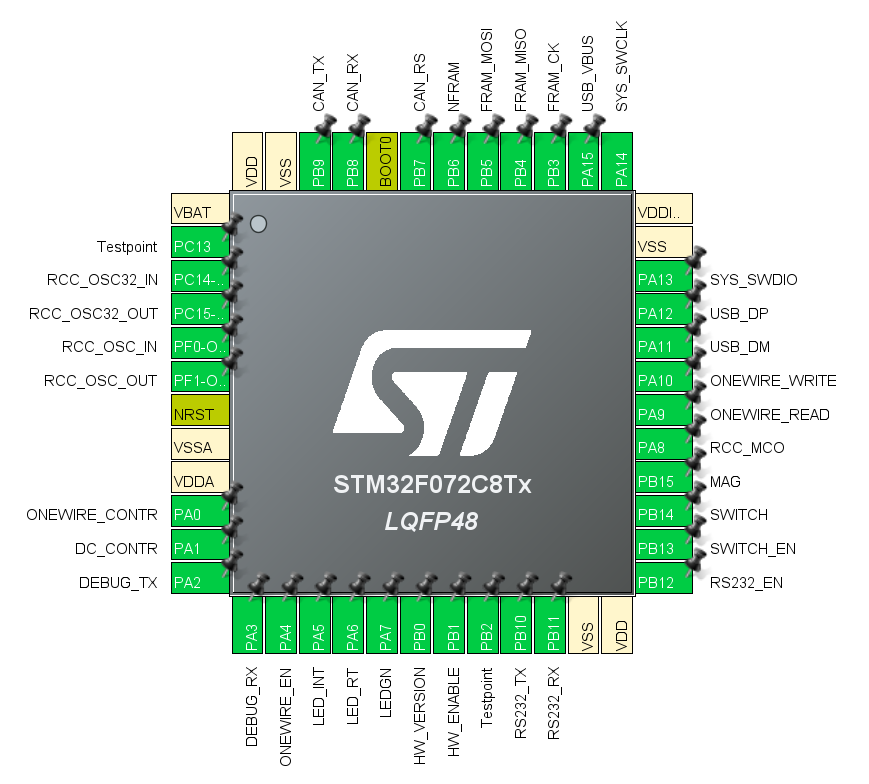
\includegraphics[width=1\textwidth]{resources/images/STMCUBE.png}
    \caption[Übersicht der Anschlüsse des Microcontrollers]{Übersicht der Anschlüsse des Microcontrollers
        (Erstellt mit STM32CubeMX\cite{stmcube})}
    \label{fig:uC_uebersicht}
\end{figure}

\paragraph{Quarze}\mbox{}\\
Der Microcontroller benötigt zwei Quarze, einen mit \(8MHz\) für den Systemtakt und einen mit \(32,768kHz\) für die \ac{RTC}.
Quarze werden direkt zwischen den entsprechenden Pins des Microcontrollers angeschlossen und mit jeweils einem Kondensator
gegen Masse beschaltet. Die Werte der Kondensatoren werden in den Datenblättern der Quarze angegeben und betragen für den
\(8Mhz\) Quarz X201 \(22pF\) und für den \(32,768kHz\) Quarz X200 \(15pF\).

Die Widerstände R204 und R205 sind beides \(0\Omega\) Widerstände, die bei eventuellen Problemen mit den Quarzen durch
Widerstände mit einem höheren Wert ersetzt werden können, um die Schwingfrequenz zu verändern.

\paragraph{Debug Schnittstelle}\mbox{}\\
Für die Entwicklung der Software wird eine Debug Schnittstelle benötigt, die es ermöglicht den Microcontroller zu programmieren
und Debug Ausgaben zu erhalten. Für diese Aufgabe ist ein 5 poliger Stecker vorgesehen, der an einem \ac{UART} des Microcontrollers
angeschlossen ist und eine Leitung zum BOOT0 Pin hat, die zum flashen neuer Software auf den Mictocontroller genutzt wird.
Die anderen beiden Pins sind für die Versorgungsspannung und die Masse.

Die Lese- und Schreibpins sind jeweils über einen Kanal des Widerstandsarrays R200 auf Versorgungsspannung gezogen, um
den Microcontroller nicht zu stören wenn der Stecker nicht eingesteckt ist. Der invertierte Programmierpin hingegen ist über zwei
Kanäle des R200 auf 3,3V gezogen, was den Pull-Up Widerstand halbiert. Alle drei Pins sind jeweils mit einem TVS Diodenpaar in 
dem Bauteil D200 gegen Über- und Unterspannung geschützt.

Über das Logikgatter U200 wird der invertierte Programmierpin wieder invertiert um mit dem BOOT0 Pin des Microcontrollers verbunden 
zu werden, der nicht invertiert ist. So wird sichergestellt, dass der Microcontroller nur in den Programmiermodus wechselt, wenn
der Stecker eingesteckt ist. 

\paragraph{Batterie}\mbox{}\\
Um die \ac{RTC} auch bei Stromausfall mit Spannung zu versorgen, wird eine Batterie angeschlossen. Mit dem
Widerstand R203 zwischen Batteriehalter und Pin des Microcontrollers wird der Strom begrenzt.
Die \(1nF\) und \(100nF\) Kondensatoren C200 und C201 sind dabei wieder als Puffer, vor allem für die Glättung
eventueller Spannungsspitzen, gedacht.

\

Über die parallelen Schottky Dioden innerhalb des D201 Gehäuses wird die Batterie nur verwendet, wenn die Versorgungsspannung
des Microcontrollers unter die Spannung der Batterie fällt. So wird verhindert, dass die Batterie entladen wird, wenn der
Automat läuft und die Batterie nicht benötigt wird.

\paragraph{Hardware Version}\mbox{}\\
Mit dem Spannungsteiler durch die Widerstände R201 und R202 wird die Hardware Version des Schlosses angegeben, sodass diese
von der Software dann erkannt werden kann und eventuelle Hardwareänderungen softwareseitig berücksichtigt werden können, ohne
ältere Versionen zu beeinträchtigen.

\begin{table}[H]
    \centering
    \begin{tabular}{cccc}
        \toprule
        Version & R202 & R201 & AD-Wandler Wert \\
        \midrule
        0       & 0    & INF  & 225             \\
        1       & 1K   & 10K  & 232             \\
        2       & 1K   & 3K9  & 203             \\
        3       & 1K   & 2K4  & 180             \\
        4       & 2K2  & 3K3  & 153             \\
        5       & 3K3  & 3K3  & 128             \\
        6       & 3K3  & 2K2  & 102             \\
        7       & 2K4  & 1K   & 75              \\
        8       & 3K9  & 1K   & 52              \\
        9       & 10K  & 1K   & 23              \\
        10      & INF  & 0    & 0               \\
        \bottomrule
    \end{tabular}
    \caption{Widerstandswerte des Spannungsteilers für verschiedene Hardware Versionen (R201 und R202 jeweils in Ohm)}
    \label{tab:hardware_version}
\end{table}

Mit dem Spannungsteiler zwischen \(3,3V\) Versorgungsspannung und Masse könnte ein Pin des Microcontrollers weniger verwendet
werden. Allerdings würde dadurch ein konstanter Strom durch R201 fließen was einerseits Energie kostet und andererseits die
Auswahl der Widerstandswerte einschränkt, da der Strom nicht zu groß werden darf. Deshalb wird der Widerstand R202
stattdessen an einen \ac{GPIO} Ausgang des Microcontrollers angeschlossen und nur bei der Abfrage der Hardware Version
eingeschaltet. So wird nur bei der Abfrage der Hardware Version Energie verbraucht. Diese Version ist fest in der Hardware 
verbaut und ändert sich dadurch nicht. Deshalb muss sie auch nur einmal abgefragt werden und kann dann in einer Variable
gespeichert werden. 

\paragraph{Stützkondensatoren}\mbox{}\\
Zwischen den vier VDD und VSS Pins des Microcontrollers sind jeweils ein \(100nF\) Kondensator und ein \(1nF\) 
Kondensator geschaltet. Diese Kondensatoren dienen wieder als Puffer für die Versorgungsspannung.
Wie bereits an verschiedenen anderen Stellen der Schaltung beschrieben, sollen sie vor allem Spannungsspitzen glätten. 
Richtwerte für die Größe dieser Kondensatoren sind in dem Datenblatt des Microcontrollers zu finden
(siehe Datenblatt S.49\cite{stm32}).

\paragraph{Testpunkte}\mbox{}\\
Der Testpunkt TP200 ist mit dem \enquote{main clock out} Pin verbunden, über den der Takt der Hauptuhr des Microcontrollers
ausgegeben wird. Dieser Pin kann verwendet werden um, die Taktfrequenz des Microcontrollers zu messen und zu überprüfen, ob
der Microcontroller richtig läuft. 

Die Testpunkte TP201 und TP202 sind mit einfachen \ac{GPIO} Ausgängen verbunden und können (vor allem bei der Entwicklung und 
Fehlersuche) verwendet werden, um Signale auszugeben und zu überprüfen, ob die Software richtig läuft. 

\paragraph{\acp{ADC}}\mbox{}\\
Die Spannung des OneWire Interfaces und die interne 30V Spannung werden über einen Spannungsteiler auf \ac{ADC} Eingänge gelegt.
Die Werte dieser Spannungen können dann von der Software ausgelesen werden, um die Spannungen zu überwachen und eventuelle
Probleme zu erkennen, oder Maßnahmen zu ergreifen. Besonders wichtig ist die Überwachung der 30V Spannung, da diese 
Spannung bei Batteriebetrieb kontinuierlich sinkt und ein kontrolliertes Herunterfahren des Systems eingeleitet werden muss,
bevor die Spannung zu niedrig wird und das System unkontrolliert herunterfährt. \\
Über den \ac{ADC} Eingang des OneWire Interfaces kann die Spannung des OneWire Busses überwacht werden unter anderem um 
herauszufinden, ob die Versorgung aktuell über diesen Bus anstatt der 24V Automatenspannung erfolgt.

Die Spannungsteiler sind so ausgelegt, dass die Referenzspannung von \(3,3V\) nicht überschritten werden sollte und die 
Ströme durch die Widerstände möglichst gering sind, um die Energieeffizienz nicht zu beeinträchtigen. \\
Der Spannungsteiler für die 30V Spannung besteht aus den Widerständen R102(\(33k\Omega\)) und R110(\(3,3k\Omega\)), die 
zusammen einen Faktor von 10:1 ergeben. \\
Der andere Spannungsteiler besteht aus den Widerständen R103(\(15k\Omega\)) und R104(\(4,7k\Omega\)), die eine 
Spannungsverhältnis von ungefähr 3:1 verursachen.

\subsection{Serielle Schnittstellen}
Die diversen seriellen Schnittstellen des Microcontrollers müssen alle entsprechend beschaltet werden um Funktion und 
Sicherheit zu gewährleisten. Die Beschaltung der einzelnen Schnittstellen wird im Folgenden kurz beschrieben.

\paragraph{OneWire}\mbox{}\\
Der OneWire Leser auf der Außenseite des Automaten wird über den zweipoligen Stecker J302 an die Platine angeschlossen.
Die Sicherung F300 und die Diode D305 sind zum Schutz der Schaltung vor Kurzschluss und Überspannung gedacht. 

Transistor T303 ist ein \ac{MOSFET}, der durch einen \ac{PWM} Ausgang des Microcontrollers angesteuert wird und die OneWire
Leitung mit Masse verbindet. Wie in Kapitel \ref{sec:one_wire} beschrieben, wird der OneWire Bus durch einen Pull-Up Widerstand
auf Versorgungsspannung gezogen. Wenn der \ac{MOSFET} leitet, wird die Leitung mit Masse verbunden und der OneWire Bus wird
auf Masse gezogen.

Transistor T301 ist ein \ac{MOSFET}, der durch einen \ac{GPIO} Ausgang des Microcontrollers angesteuert wird und schaltet 
den besagten Pull Up Widerstand. Dies ist im Vergleich zu Version 1.0 eine Neuerung, die es ermöglicht den OneWire Bus
bei Bedarf abzuschalten. Wenn kein OneWire gerät angeschlossen ist, wird dieser periodisch an und ausgeschaltet, um Energie
zu sparen und die Lebensdauer des OneWire Lesers zu erhöhen, der sonst ständig mit Spannung versorgt würde und dadurch 
schneller Korrodiert.

Die read-Leitung ist durch Widerstand R312 strombegrenzt und mit einem \enquote{direct capture} Timer Pin des Microcontrollers
verbunden.  

\paragraph{\ac{USB}}\mbox{}\\
Als \ac{USB} Anschluss wird ein Picoblade Stecker S401 verwendet, im Gegensatz zu den \ac{USB} standard Steckern, da dieser 
Stecker besser für diese Anwendung geeignet ist. Die Anschlüsse dieses Steckers sind mit der TVS Diode D400 gegen ESD Probleme
geschützt. \\
\ac{USB} Plus und \ac{USB} Minus Leitungen werden über die Kombodrossel L400 weiterhin gegen Störungen geschützt und dann direkt 
an die entsprechenden Pins des Microcontrollers angeschlossen.

\ac{USB} VBus wird über den Spannungsteiler mit den Widerständen R402 und R403 auf einen \ac{GPIO} Eingang des Microcontrollers
gelegt. Dieser Spannungsteiler dient dazu, die 5V Versorgungsspannung des \ac{USB} Anschlusses auf die 3,3V des Microcontrollers
zu reduzieren, um die Schaltung nicht zu beschädigen.

Die Kabel einer \ac{USB} Verbindung haben ein Schirmgeflecht, welches es vor elektromagnetischen Störungen schützt. Dieses 
Schirmgeflecht liegt an dem SHIELD Pin des \ac{USB} Steckers an und wird über den Widerstand R409 parrallel zu Kondensator 
C405 mit Masse verbunden. 

\paragraph{RS232}\mbox{}\\
Die RS232 Schnittstelle wird über die RJ45 Buchse J400 angeschlossen. Zwischen den Pins der Buchse und den Pins des Microcontrollers
ist der RS232 Treiber U400 geschaltet, der die Signale auf die richtigen Pegel bringt.

Dieser Treiber wird nach den Angaben des Datenblattes beschaltet (siehe Datenblatt \cite{max3221}) und mit einem entsprechendem 
Stützkondensator versehen. Die TXD Leitung ist mit einem \(10k\Omega\) Pull-Up Widerstand auf Versorgungsspannung und 
die Enable Leitung ist mit einem \(10k\Omega\) Pull-Down Widerstand auf Masse gezogen.

\paragraph{CAN}\mbox{}\\
Für dem \ac{CAN} Bus wird der \ac{CAN} Transceiver U402 verwendet. Um den, im Standard gegebenen, \(120\Omega\) 
Abschlusswiderstand zu erreichen, werden zwei \(61,9\Omega\) Widerstände R406 und R407 in Reihe geschaltet. Zwischen
diesen Widerständen ist der Kondensator C404 mit einer Kapazität von \(4,7\mu F\) gegen Masse angeschlossen. Dieser Kondensator
verbessert EMI Verhalten und stabilisiert die Spannung des Busses. Mit der Kombodrossel L401 wird der Bus weiterhin gegen 
Störungen geschützt.

Die Datenleitungen TX und RX zwischen Microcontroller und Treiber sind wieder mit \(4,7k\Omega\) Pull-Up Widerständen auf
Versorgungsspannung gezogen. Die Enable Leitung ist mit einem \(4,7k\Omega\) Pull-Down Widerstand auf Masse gezogen.

\paragraph{SWD}\mbox{}\\
Der 5 Polige \ac{SWD} Stecker J400, der für die Programmierung und Debugging des Microcontrollers verwendet wird, ist direkt
mit den entsprechenden Pins des Microcontrollers verbunden. SWDIO ist mit einem \(4,7k\Omega\) Pull-Down Widerstand auf Masse
gezogen, während SWCLK sowie NRST mit einem \(4,7k\Omega\) Pull-Up Widerstand auf Versorgungsspannung gezogen ist. 

\subsection{Sonstige Bauteile}
In diesem Abschnitt werden die Bauteile und Schaltungen beschrieben, die nicht in die anderen Kategorien passen.

\paragraph{\ac{FRAM}}\mbox{}\\
Der \ac{FRAM} Speicher wird über ein \ac{SPI} verbunden. Der \ac{GPIO} Ausgang \enquote{NFRAM} des Microcontrollers wird verwendet,
um den Speicherbaustein zu deaktivieren. \\
Während die Clock-Leitung mit einem Pull-Down Widerstand auf Masse gezogen ist, sind die Datenleitungen und NFRAM mit \(4,7k\Omega\)
auf 3,3V gezogen.

\paragraph{LEDs}\mbox{}\\
Es werden drei \acp{LED} vorgesehen, von denen sich eine auf dem \ac{pcb} befindet und zwei weitere über einen Stecker angeschlossen
werden können. Alle drei \acp{LED} können über ein \ac{PWM} Signal vom Microcontroller angesteuert werden um die Helligkeit zu
regulieren. \\
Die beiden \acp{LED} die über einen dreipoligen Stecker angeschlossen werden können, sind jeweils mit einem TVS Diodenpaar im Bauteil 
D301 gegen Über- bzw. Unterspannung geschützt. 

Durch das Ansteuern der \acp{LED} über die Kathode wird, im Gegensatz zu einer Schaltung an die Anode mit der Kathode auf Masse, 
weniger Last auf die Ausgänge des Microcontrollers gelegt. Das sorgt für eine stabilere Schaltung und schont den Microcontroller.

Durch die verschiedenen Vorwiderstände R300, R301 und R302 können die \acp{LED} mit verschiedenen Strömen betrieben werden:
\begin{itemize}
    \item \textbf{R300:} \(1k\Omega\) \(\rightarrow\) \(3,3mA\)
    \item \textbf{R301:} \(470\Omega\) \(\rightarrow\) \(7mA\)
    \item \textbf{R302:} \(330\Omega\) \(\rightarrow\) \(10mA\)
\end{itemize}

\paragraph{Schalter}\mbox{}\\
Ein Endschalter um zu erkennen, in welchem Zustand sich der Schlossriegel befindet, kann über den zweipoligen Stecker S301
angeschlossen werden. Mit der Enable Leitung kann der Endschalter aktiviert und deaktiviert werden, um den Stromverbrauch
zu reduzieren wenn der Endschalter nicht benötigt wird. 

Wenn der Endschalter geschlossen ist fließt die Spannung des Enable Pins über den Widerstand R304 auf Masse und am 
Detect Pin liegen \(0V\) an. Wenn der Endschalter geöffnet ist, fließt kein Strom mehr und die Spannung des Enable Pins
liegt an dem Detect Pin an. 

Um Schalterprellen zu verhindern, wird der Detect Pin mit einem \(100nF\) Kondensator C301 gegen Masse geschaltet. Dieser
soll die Spannung glätten. Außerdem ist der Stecker mit einer \(3,3V\) TVS Diode D302 gegen Überspannung geschützt.

\paragraph{Magnet}\mbox{}\\
Über den Widerstand R310 wird der Strom zur Basis des \ac{MOSFET} T302 begrenzt, Widerstand R313 ist ein \(10k\Omega\) Pull-Down.
Wenn an der \enquote{MAG} Leitung ein Signal anliegt, wird der \ac{MOSFET} T302 leitend und somit bildet sich ein 1:1 Spannungsteiler
mit den \(10k\Omega\) Widerständen R307 und R308. Dadurch wird die Gate-Source Spannung des P-Kanal \ac{MOSFET} T300 negativ 
und dieser beginnt zu leiten, womit die interne 30V Spannung an den Stecker für den Magneten angelegt wird. \\
Mit der TVS-Diode D303 wird die Schaltung gegen Überspannung geschützt.

Durch diese Schaltung wird der Magneten nur aktiviert wenn ein Signal an der \enquote{MAG} Leitung anliegt. Es entstehen keine
Verlustleistungen und die hohe Spannung wird sicher geschalten.

\clearpage

\section{Layout}
Nachdem ein Schaltplan erstellt ist, müssen die Bauteile auf einer Platine angeordnet werden. Im Folgenden wird das Layout der
Platine beschrieben und der Prozess dahinter erläutert.

\subsection{Physikalischer Aufbau}
Das Layout der Platine wurde mit dem Programm \enquote{Altium Designer} erstellt. Die Platine ist vierlagig und hat eine Größe
von \(75mm \times 76mm\). Die oberste Lage ist die Signallage, die zweite Lage ist die Massefläche, die dritte Lage ist die
Versorgungsspannung und die unterste Lage ist die Signallage. In den Ecken befinden sich Bohrungen mit einem Durchmesser von
\(3,5mm\), die für die Befestigung der Platine im Gehäuse verwendet werden. Die Stecker, die aus der Version 1.0 übernommen 
wurden sind entsprechend an den gleichen Stellen angeordnet. 

Diese äußeren Merkmale sind wegen der Anforderung nach Rückwärtskompatibilität durch die aktuelle Version festgelegt und können 
nicht verändert werden.

Die Leiterbahnen, die nicht explixit größer sein sollten, haben alle eine Breite von 0.253mm (10 thou). Die Vias, die verschiedene 
Lagen des \ac{pcb} miteinander verbinden haben einen Durchmesser von \(0,7mm\), einen Loch-Durchmesser von \(0,3mm\) und einen 
Abstand von \(0,2mm\) zu den Leiterbahnen.

\subsection{Vorgehensweise}
Zuerst werden die Bauteile auf der Platine platziert. Dabei ist es besonders
wichtig, Komponenten die hohe Ströme oder Hochfrequente Signale brauchen zu beachten. Eine Gruppierung nach Funktion ist sinnvoll, 
um die Bauteile die im Zusammenhang stehen möglichst nah beieinander zu platzieren.

\

Nachdem die Komponenten platziert sind, werden die Leitungen zwischen den ihnen geroutet. Dabei ist es wichtig, dass die Leitungen
möglichst kurz sind und eine angemessene Dicke haben, um die Ströme zu führen, die durch sie fließen. Außerdem sollten Leitungen 
nicht zu nah an störanfälligen Bauteilen und Leitungen vorbeigeführt werden, um Störungen zu vermeiden. \\
Das verwendete Programm bietet die Möglichkeit die Leitungen automatisch zu routen, allerdings ist das Ergebnis dieser Funktion
nicht immer zufriedenstellend und muss manuell nachbearbeitet werden. Deshalb wurde die Funktion nur für die Leitungen verwendet,
die nicht kritisch sind und deshalb nicht manuell gezogen werden mussten.

Eine möglichst große Massefläche verbessert die allgemeine Störfestigkeit der Schaltung und kann am Ende des Routings hinzugefügt
werden. 

\subsection{\ac{SEPIC} Wandler}
Der \ac{SEPIC} Wandler ist ein sehr empfindlicher Teil der Schaltung, der aus vielen verschiedenen Bauteilen besteht. 
Teilweise arbeitet er mit hohen Strömen und hochfrequenten Signalen und neigt deshalb besonders dazu Störungen zu verursachen. 

Angelehnt an die Platine der Version 1.0 wurden die großen Kondensatoren C126, C126 und C127 am unteren Rand der Platine platziert.
Um die 30V Spannung möglichst in einer Region zu halten, wird der \ac{SEPIC} Wandler so nah wie möglich über diese Kondensatoren
platziert. Bei der Platzierung ist der Eingang des Wandlers natürlich auch ein wichtiger Faktor. Da sich die Eingänge für die 
24V Automatenspannung am linken Rand der Platine befinden und der OneWire Leser am rechten Rand, wurde der Wandler einigermaßen 
in der Mitte platziert.

Bei der Anordnung der Bauteile wurde sich an den Layout Empfehlungen des Datenblattes orientiert (siehe Datenblatt S.34 \cite{LM5157}).
So werden die AGND und DGND Flächen getrennt und am AGND Pin des Reglers zusammengeführt. Der schaltende Kreis ist so klein wie 
möglich und die stromführenden Leitungen sind breit genug, um die Ströme zu führen, die durch sie fließen.

Unter der Doppelspule L100 setzt die Massefläche aus und wurde weitestgehend verhindert Leitungen unter der Spule zu führen, um
Störungen durch die hochfrequent schaltende Spule zu vermeiden. Eine weitere Maßnahme um Störungen zu vermeiden ist das 
physikalische trennen der Masseflächen von dem Schaltregler und dem Rest der Schaltung und das Aussetzen der Versorgungslage
unter dem gesamten Schaltregler. Somit kann einerseits keine Schwingung auf diese Ebene übertragen werden und andererseits
kann die Schicht dadurch als weitere GND Fläche verwendet werden, um mehr Hitze von den Bauteilen abzuleiten.

\subsection{Buck Wandler}
Bei der Platzierung des Buck Wandlers ist nur darauf zu achten, dass keine lange 30V Leitung entsteht. Da der Ausgang des 
Schaltreglers direkt auf die Versorgungslage gegeben wird, orientiert sich die Platzierung nur an der Position der Eingänge.

Hier wird sich ebenfalls an der Layout Empfehlung des Datenblattes orientiert (siehe Datenblatt S.34 \cite{AP63203WU}). 
Bei der Platzierung der Eingangskondensatoren wird darauf geachtet die Kondensatoren mit der niedrigsten Kapazität am nächsten
an den Eingang zu platzieren, da diese Kondensatoren die höchsten Frequenzen glätten müssen.

Die Versorgungslage wird auch bei diesem Wandler unter den schaltenden Elementen ausgesetzt, um diese vor den entstehenden 
Schwingungen zu schützen. Des weiteren wird die Massefläche des Wandlers unter der Spule ausgesetzt und von der restlichen
Massefläche, aus oben genannten Gründen, getrennt.

\subsection{Quarz Oszilatoren}
Eine der empfindlichsten Stellen der Schaltung sind die Quarze, die für die Takterzeugung verwendet werden. Diese Bauteile
sind sehr störungsanfällig und müssen deshalb besonders sorgfältig platziert werden. Durch die hohe Frequenz
der Signale, die durch diese Bauteile übertragen werden ist es besonders wichtig, die Leitungen zwischen den Bauteilen
möglichst kurz zu halten und die Quarze möglichst nah an den entsprechenden Pins des Microcontrollers zu platzieren.

Auch hier wird die lokale Massefläche von der restlichen Massefläche getrennt, um Störungen zu
verhindern. Zusätzlich wurde die Masselage unter den Quarzen isoliert und nur an einer Stelle mit der restlichen Masselage
verbunden, um die Schwingungen der Quarze nicht auf die restliche Lage zu verteilen.

\subsection{\ac{USB} Anschluss}
Für eine stabile und störungsfreie \ac{USB} Verbindung ist es wichtig, dass die Datenleitungen zwischen dem \ac{USB} Anschluss und
dem Microcontroller möglichst gleich lang und am besten auch parallel zueinander verlaufen. Deshalb wurde der \ac{USB} Stecker
direkt neben dem Microcontroller platziert und die Datenleitungen möglichst gerade und parallel zueinander geroutet.

Für einen optimalen Schutz gegen Störungen wurde darauf geachtet die Datenleitungen möglichst weit von anderen Leitungen zu führen
und keine hochfrequenten Verbindungen unter diesen Leitungen zu führen. Die TVS Diode ist direkt neben dem \ac{USB} Stecker platziert,
sodass die Überspannung direkt an der Quelle abgefangen wird und sich nicht weiter auf die Schaltung auswirken kann. 

Die Komponenten des SHIELD Pins sind außerdem so nah wie möglich an dem \ac{USB} Stecker platziert, um die Störungen die durch das
Schirmgeflecht der \ac{USB} Kabel entstehen können nicht auf der Platine zu verteilen.

\clearpage

\section{Verbesserungen gegen alte Version}
Die Version 2.0 der Platine ist eine Weiterentwicklung der Version 1.0, die einige Verbesserungen und neue Funktionen mit sich bringt.
Im Folgenden werden die wichtigsten Verbesserungen und Neuerungen beschrieben.

\subsection{Neue Funktionen}
In der neuen Version werden einige neue Funktionen hinzugefügt, die entweder in der Nutzung der Platine aufgefallen sind, oder
die in Zukunft benötigt werden.

\paragraph{OneWire Abschaltung}\mbox{}\\
In der Version 1.0 wird der OneWire Leser ständig mit Spannung versorgt, was dazu führt, dass der Leser schneller korrodiert
und die Lebensdauer des Lesers verkürzt wird. Deshalb wird in der Version 2.0 der OneWire Leser nur noch bei Bedarf mit Spannung 
versorgt.

\paragraph{Hardware Version}\mbox{}\\
Die Hardware Version wird im Gegensatz zur alten Platine nun durch fest verbaute Widerstände auf der Platine angegeben und kann 
von der Software ausgelesen werden um entsprechende Parameter anzupassen.

\paragraph{\ac{CAN} Bus}\mbox{}\\
Eine weiter Neuerung ist die \ac{CAN} Schnittstelle, die bei anderen krauth technology Produkten bereits Standard und auch
bei dem E-Schloss durchaus sinnvoll ist. Alle Automaten Komponenten einheitlich über \ac{CAN} zu verbinden bietet viele Vorteile
wie eine einfache Verkabelung und eine einheitliche Kommunikation zwischen den Komponenten.

\paragraph{Endschalter}\mbox{}\\
Die Möglichkeit einen Endschalter des Schlossriegels anzuschließen wurde hinzugefügt, um den Zustand des Schlosses festzustellen
und eventuelle Probleme zu erkennen.

\subsection{Veränderungen}
Neben den neuen Funktionen wurden auch einige Veränderungen an der Platine vorgenommen, um die Schaltung zu verbessern und
die Fehler/Probleme der alten Platine zu beheben.

\paragraph{Microcontroller}\mbox{}\\
Der Grund für die Entwicklung einer neuen Platine ist die Tatsache, dass der alte Microcontroller nicht mehr verfügbar ist.
Der neue STM32F072C8T6 ist ein modernerer Microcontroller mit mehr Funktionen und vor allem einer garantierten Verfügbarkeit
von 10 Jahren.

\paragraph{Spannungsversorgung}\mbox{}\\
Die Spannungsversorgung wurde komplett überarbeitet, um die Schaltung effizienter zu machen und auch stärkere Magneten mit 
mehr Spannung betreiben zu können. Die aktuellen Magneten können über eine \ac{PWM} Spannung von \(30V\) ebenfalls betrieben
werden, was die rückwärtskompatibelität gewährleistet.

\paragraph{Energiespeicher}\mbox{}\\
Durch die eben beschriebene Überarbeitung der Spannungsversorgung wurde auch der Energiespeicher überarbeitet. Die alte Version
verwendete \(3 \times 4700\mu F\) Kondensatoren, bei 12V Spannung entspricht das einer gespeicherten Energie von \(1,01J\). 
Mit der neuen Version werden \(3 \times 2200\mu F\) Kondensatoren bei 30V Spannung verwendet, was mit einer Energie von \(2.97J\) 
fast einer Verdreifachung entspricht.

\paragraph{Programmier Interface}\mbox{}\\
Der \ac{JTAG} Stecker wurde durch einen \ac{SWD} Stecker ersetzt. \ac{SWD} ist ein simpler und moderner Standard, der
weniger Pins als \ac{JTAG} benötigt und dennoch alle erforderlichen Funktionen mit sich bringt. 

\paragraph{Speicher}\mbox{}\\
Die Kapazität des \ac{FRAM} Speichers wurde von \(8 \times 8kbit\) auf \(8 \times 32kbit\) vergrößert, um mehr Daten speichern 
zu können. Der Wunsch nach mehr Speicherplatz ist im Betrieb des aktuellen E-Schlosses aufgekommen und kann bei der neuen Version
sehr einfach erfüllt werden.

\paragraph{\ac{RTC}}\mbox{}\\
Von dem externen \ac{RTC} Bauteil wurde abgesehen und stattdessen der interne \ac{RTC} des Microcontrollers verwendet. Dies ist
platzsparender und einfacher zu implementieren, da weniger zusätzlichen Bauteile benötigt werden.